%! TeX program = lualatex
\documentclass[a4paper,11pt]{article} 
% packages
\usepackage{censor}
\StopCensoring
\usepackage{fontspec}
\setmainfont{EB Garamond}
% for tironian et fallback
% % \directlua{luaotfload.add_fallback
% % ("emojifallback",
% %      {"Noto Serif:mode=harf"}
% % )}
% % \setmainfont{EB Garamond}[RawFeature={fallback=emojifallback}]

\setmonofont[Scale=MatchLowercase]{Deja Vu Sans Mono}
\usepackage[a4paper,left=2cm,right=2cm,top=\dimexpr15mm+1.5\baselineskip,bottom=2cm]{geometry}
\setlength{\parindent}{0pt}

\usepackage{fancyhdr}       % Headers and footers 
\fancyhead[R]{\normalfont \leftmark}
\fancyhead[L]{}
\pagestyle{fancy}
\usepackage{amsmath}

\usepackage{microtype}      % Slightly tweak font spacing for aesthetics
\usepackage{multicol}
\usepackage[english]{babel} % Language hyphenation and typographical rules
\usepackage{xcolor}
\definecolor{linkblue}{RGB}{0, 64, 128}
\usepackage[final, colorlinks = false, urlcolor = linkblue]{hyperref} 
% \newcommand{\secref}[1]{\textbf{§~\nameref{#1}}}
\newcommand{\secref}[1]{\textbf{§\ref{#1}~\nameref{#1}}}

\usepackage{changepage}     % adjust margins on the fly

\usepackage{minted}
\usemintedstyle{algol_nu}

\usepackage{pgfplots}
\pgfplotsset{width=\textwidth,compat=1.9}

\usepackage{caption}
\newenvironment{code}{\captionsetup{type=listing}}{}
\captionsetup[listing]{skip=0pt}
\setlength{\abovecaptionskip}{5pt}
\setlength{\belowcaptionskip}{5pt}

\usepackage[yyyymmdd]{datetime}
\renewcommand{\dateseparator}{--}

\usepackage{enumitem}

\usepackage{titlesec}

\author{Andrew Hayes}

\begin{document}
\begin{titlepage}
    \begin{center}
        \hrule
        \vspace*{0.6cm}
        \censor{\huge \textbf{CT436}}
        \vspace*{0.6cm}
        \hrule
        \LARGE
        \vspace{0.5cm}
            Advanced Professional Skills
        \vspace{0.5cm}
        \hrule

        \vfill
        \vfill

        \hrule
        \begin{minipage}{0.495\textwidth} 
            \vspace{0.4em}
            \raggedright
            \normalsize 
            Name: Andrew Hayes \\
            E-mail: \href{mailto://a.hayes18@universityofgalway.ie}{\texttt{a.hayes18@universityofgalway.ie}}  \hfill\\   
            Student ID: 21321503 \hfill
        \end{minipage}
        \begin{minipage}{0.495\textwidth} 
            \raggedleft
            \vspace*{0.8cm}
            \Large
            \today
            \vspace*{0.6cm}
        \end{minipage}
        \medskip\hrule 
    \end{center}
\end{titlepage}

\pagenumbering{roman}
\newpage
\tableofcontents
\newpage
\setcounter{page}{1}
\pagenumbering{arabic}

\section{Introduction}
\subsection{Lecturer Contact Information}
\begin{itemize}
    \item   Dr. Owen Molloy (\href{mailto://owen.molloy@universityofgalway.ie}{\texttt{owen.molloy@universityofgalway.ie}}
\end{itemize}

\subsection{Group Project}
\begin{itemize}
    \item   Groups of 3 -- 5.
    \item   Work on an idea that your team is excited about.
    \item   Take the ideation \& team formation phase very seriously: it can greatly determine your experience
            within the class.
    \item   If you find that your idea hits a dead-end, do not be afraid to pivot mid-way through the semester.
\end{itemize}

Each team will maintain an online portfolio documenting their journey \& linking with or containing their deliverables:
\begin{multicols}{2}
\begin{itemize}
    \item   Idea generation.
    \item   Market segmentation / analysis.
    \item   End-user profiling.
    \item   Customer persona.
    \item   Lifecycle use case.
    \item   Quantified value proposition.
    \item   Product brochure.
    \item   Business model canvas / business plan.
    \item   Video (which will be submitted to EI Student Entrepreneur Awards).
\end{itemize}
\end{multicols}

\subsection{Expected Module Deliverables}
Exact details \& order for the following are still to be finalised, but will largely follow previous years:
\begin{itemize}
    \item   Portfolio: for documenting the project, meetings, showing how ideas have advanced. (15\%).
    \item   Video (25\%).
    \item   Product brochure, QVP (Quantified Value Proposition), \& (customer) Persona(e) (20\%).
    \item   EI Template (Basic Business Plan) (30\%).
    \item   Submit video to EI student Entrepreneur awards (5\%).
    \item   Attendance (5\%).
\end{itemize}

\section{Innovation}
\textbf{Innovation} consists of using new technology \& new ways of thinking to add value to an existing idea or
product and to make substantial changes in society.
Innovation = Invention $\times$ Commercialisation.

\subsection{Four Misinterpretations of Innovation}
\begin{enumerate}
    \item   \textbf{Innovation $\neq$ Invention}: An invention is a creative idea while an innovation makes that idea 
            feasible and turns it into a product or service that satisfies the customer's needs.

    \item   \textbf{Innovation $\neq$ New Products and/or Services}: Innovation has rightly been associated with many 
            cases of new product development.
            However, innovation can concern other new developments such as new markets or new marketing methods.

    \item   \textbf{Innovation $\neq$ Original}: Innovation often builds on old existing ideas \& resources.
    
    \item   \textbf{Innovation $\neq$ One-Off Inspiration}: Unlike the one sudden flash of inspiration, innovation
            is a gradual process that takes place over a period of time (or incubation).
\end{enumerate}

\subsection{Sources of Innovation}
Innovators are generally attentive to changes which give them clues to what opportunities may come in future.
Would-be innovators must also go out and look, ask, \& listen.
Above all, innovation is \textit{work} rather than \textit{genius}.
It requires knowledge, it requires focus, and it often requires integrity.

\begin{figure}[H]
    \centering
    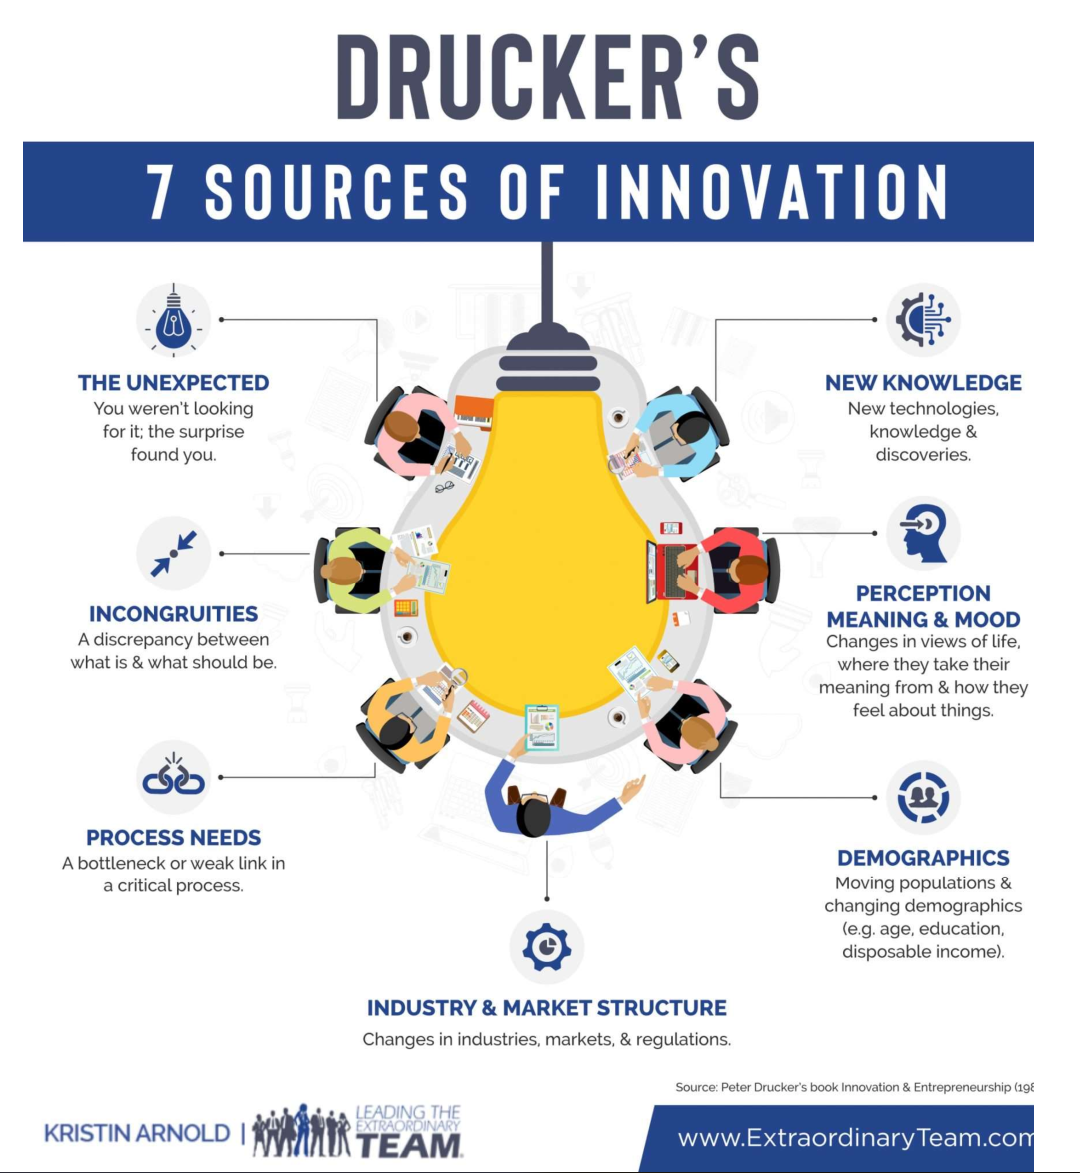
\includegraphics[width=0.6\textwidth]{images/druckers_sources_of_innovation.png}
    \caption{Drucker's Sources of Innovation}
\end{figure}

\subsection{Types of Innovation}
\begin{itemize}
    \item   \textbf{Invention:} Totally new product, service, or process.
    \item   \textbf{Extension:} New use or different application of an already existing product, service, or process.
    \item   \textbf{Duplication:} Creative replication of an existing concept.
    \item   \textbf{Synthesis:} Combination of existing concepts \& factors into a new formulation or use.
\end{itemize}

\section{Entrepreneurship}
\textbf{Entrepreneurship} is the formation of a new venture that produces a product or offering that creates some value to 
make it economically sustainable.
It has the ability to improve standards of living \& create wealth.

$$
\text{Innovation} = \text{Invention} \times \text{Commercialisation}
$$

In contemporary markets, entrepreneurs act as innovators or developers who identify \& capture opportunities, transform 
the opportunities into merchandisable concepts, create value through multiple stakeholders \& resources, and take risks 
while seeking rewards for their ventures \& efforts.


\subsection{What do you need to start a successful new venture?}
\begin{enumerate}
    \item   Idea.
    \item   Team.
    \item   Process.
\end{enumerate}

Good entrepreneurial business ideas are:
\begin{enumerate}
    \item   \textbf{Market-Driven:}
            \begin{itemize}
                \item   Solve a problem.
                \item   Find a market need.
                \item   Customer-focused, not product-driven.
                \item   Targets an identified sizeable market segment.
            \end{itemize}
    \item   \textbf{Feasible:}
            \begin{itemize}
                \item   Attractive: there is a demand.
                \item   Achievable: it can be done.
                \item   Durable: it lasts.
                \item   Value-Creating: it is worth something.
                \item   Safe.
                \item   Affordable.
            \end{itemize}
    \item   \textbf{Unique:}
            \begin{itemize}
                \item   Faster/Better/Cheaper.
                \item   Differentiated (vs. commodity).
            \end{itemize}
    \item   \textbf{Fundable:}
            \begin{itemize}
                \item   Revenue stream.
                \item   Management risk.
                \item   Sustainable: market exists with frequency of purchase.
                \item   Scaleable or replicable.
                \item   Barriers to entry.
                \item   Growth potential.
                \item   Product pipeline.
                \item   Exit plan.
                \item   Innovative.
            \end{itemize}
    \item   \textbf{Innovative:}
            \begin{itemize}
                \item   Invention: totally new product/service/process.
                \item   Extension: new use or different application of an already existing product/service/process.
                \item   Duplication: creating a replication of an existing concept.
                \item   Synthesis: combining existing concepts and/or factors into new formula for use.
            \end{itemize}
\end{enumerate}

\begin{figure}[H]
    \centering
    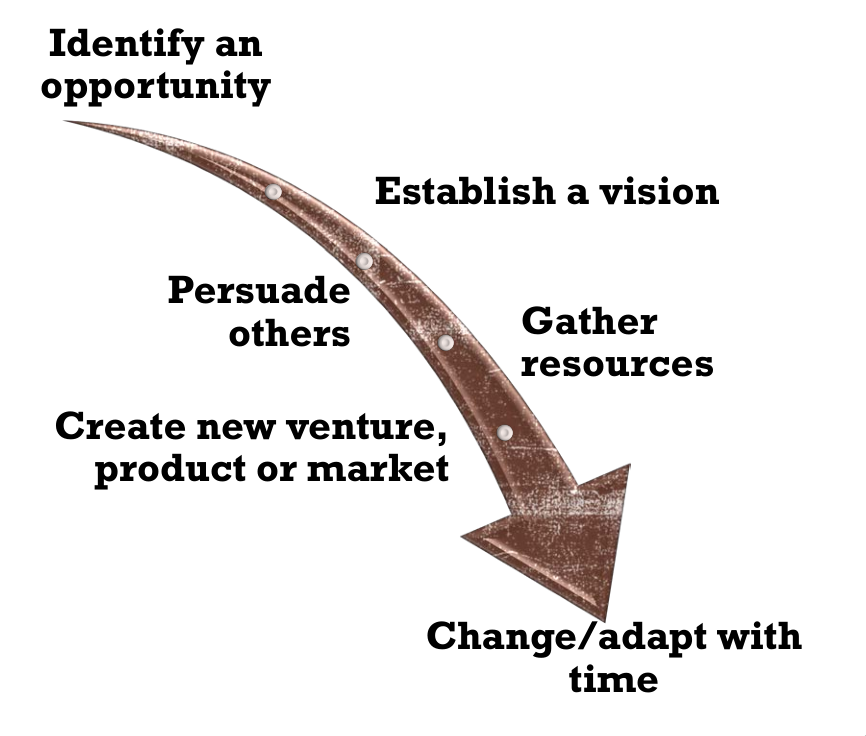
\includegraphics[width=0.8\textwidth]{images/entrepreneurial_process.png}
    \caption{The Entrepreneurial Process}
\end{figure}

\begin{figure}[H]
    \centering
    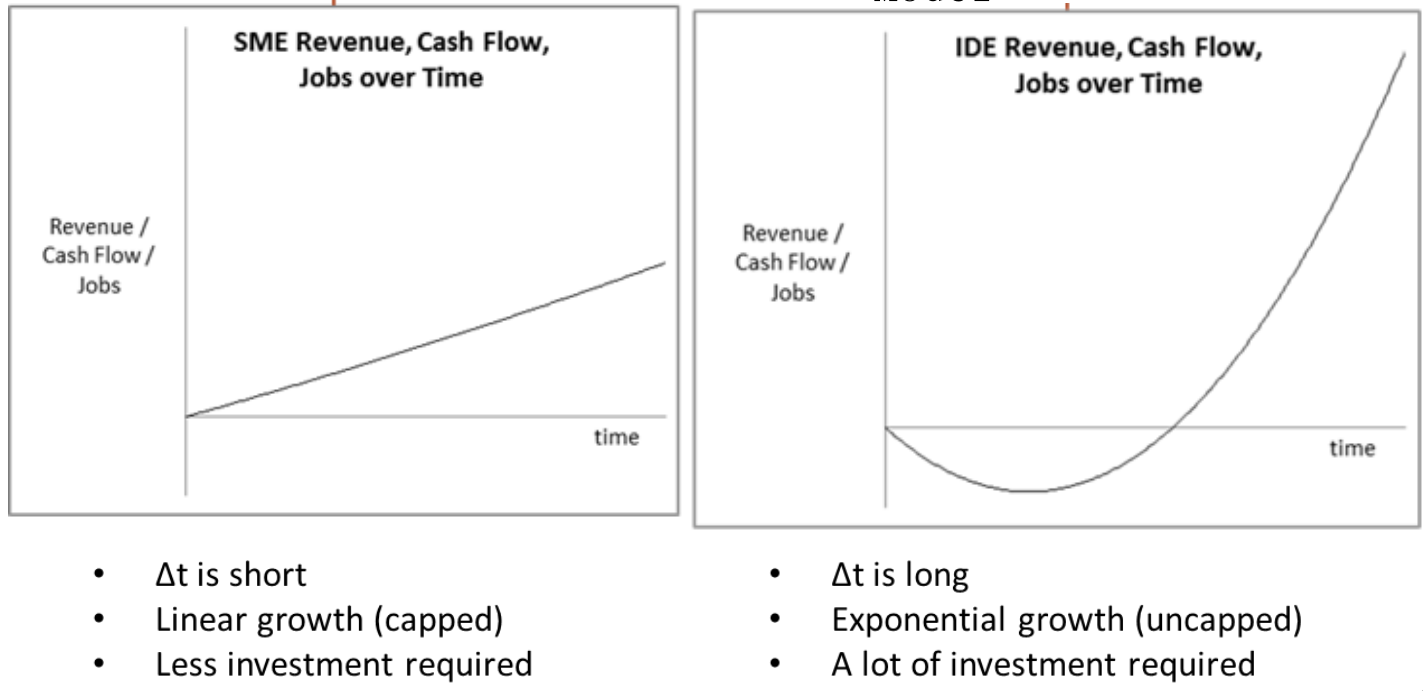
\includegraphics[width=0.8\textwidth]{images/existing_vs_innovation.png}
    \caption{``Existing Business'' Model vs Innovation-Based ``New Business'' Model}
\end{figure}

\subsection{Can Entrepreneurship be Taught?}
Entrepreneurship is:
\begin{itemize}
    \item   \textbf{Accessible:} it is not something that is available only to a gifted few.
    \item   \textbf{Learnable:} it consists of a number of fundamental skills that can be taught \& learned.
    \item   \textbf{Based on valuing unique products:} its goal is to make something new \& valued.
    \item   \textbf{Built on fundamental concepts:} it consists of basic principles which improve your chances of 
            success.
    \item   \textbf{Best learned through Apprenticeship:} best learned when theory is combined with apprenticeship-style 
            training.
\end{itemize}

\subsection{Teamwork}
Teams have a collective I.Q.
In general, good teams all share these two qualities:
\begin{itemize}
    \item   Members speak in roughly the same proportion, i.e. ``equality in distribution of conversational turn-taking''.
    \item   Members all have high ``average social sensitivity'', i.e. skill at intuiting how others felt based on their 
            tone of voice, their expressions, \& other non-verbal cues etc.
\end{itemize}

\subsubsection{Psychological Safety}
In her TEDx talk, Edmondson offers three simple things individuals can do to foster team psychological safety:
\begin{itemize}
    \item   Frame the work as a learning problem, not an execution problem.
    \item   Acknowledge your own fallibility.
    \item   Model curiosity \& ask lots of questions.
\end{itemize}

To measure a team's level of psychological safety, Edmondson asked team members how strongly they agreed or disagreed with
these statements:
\begin{itemize}
    \item   If you make a mistake on this team, it is often held against you.
    \item   Members of this team are able to bring up problems \& tough issues.
    \item   People on this team sometimes reject others for being different.
    \item   It is safe to take a risk on this team.
    \item   It is difficult to ask other members of this team for help.
    \item   No-one on this team would deliberately act in a way that undermines my efforts.
    \item   Working with members of this team, my unique skills \& talents are valued \& utilised.
\end{itemize}
 
\subsection{EI Business Plan}
\subsubsection{Product or Service}
\begin{itemize}
    \item   \textbf{Product or service:} What is the company proposing to do and what problem does it solve?
            Can you describe the products/services it will offer?
            How is this different to what is currently available on the market or how does it improve a current product?
    \item   \textbf{Future plans:} Are there plans to develop the product(s) or service(s), or add new product(s) or 
            service(s) in the future?
            How advanced is the project idea/business?
            How much work is required  to take the project to the next stage?
\end{itemize}

\subsubsection{Marketing}
\begin{itemize}
    \item   \textbf{Market Research:} Describe how the market research was carried out \& give examples. 
            Describe the market size \& number of possible customers.
    \item   \textbf{Customers:} Who are your customers?
            How do you know they are interested in your products and what their spending behaviours are?
            What are their needs/wants? 
            What is your unique selling point?
    \item   \textbf{Market trends or issues:} Describe trends or key issues anticipated in the market that may affect
            the marketplace.
    \item   \textbf{Competitors:} Who are the competitors and what are their strengths \& weaknesses?
\end{itemize}

\subsubsection{Intellectual Property}
\begin{itemize}
    \item   \textbf{Intellectual Property:} Have you legally protected your product/service to date?
            Are you aware of any other patents, trademarks, or copyright issues with your product?
    \item   \textbf{People:} What is the potential for employment in Ireland in this company?
\end{itemize}

\subsection{Creativity}
\textbf{Creativity} is anything that is new, useful, or surprising.
Artistry is not a necessary condition for creativity.
When engaging in creative problem-finding \& solving, it is important you consider:
\begin{itemize}
    \item   \textbf{Relevance:} the degree to which your solution actually solves the problem.
    \item   \textbf{Value:} importance to the customer (or to the creator).
    \item   \textbf{Novelty:} originality.
\end{itemize}

\subsubsection{Combinational Creativity}
A common misconception is that creativity cannot be cultivated, and that instead some lucky people have an innate sense of
creativity.
Creative people are often seen as a rarity: smart, curious, \& able to look at the world with fresh eyes.
According to classical psychology research, there are three main types of creativity:
\begin{itemize}
    \item   \textbf{Exploratory:} generating new ideas within a given space.
    \item   \textbf{Transformational:} ignoring fundamental rules to come up with potentially impossible but highly creative
            ideas.
    \item   \textbf{Combinational Creativity:} combining old ideas to come up with something new.
\end{itemize}

The \textbf{cone of plausibility} is a useful tool in exploring possibilities.
\begin{figure}[H]
    \centering
    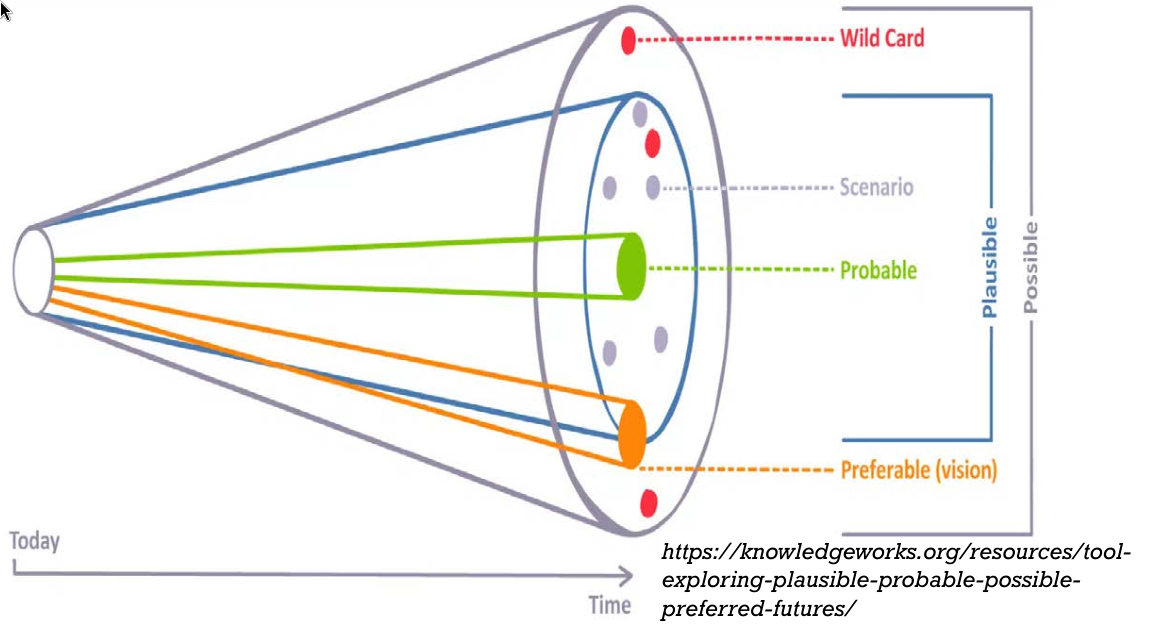
\includegraphics[width=0.8\textwidth]{images/cone.png}
    \caption{Cone of Plausibility}
\end{figure}

\section{Idea Generation Techniques}
A process for generating ideas generally follows the flow of:
$$
\text{Define your problem } \rightarrow \text{Agree judging criteria } \rightarrow \text{Set restrictions}
$$

The problem is often to know what the problem is:
\begin{itemize}
    \item   Rephrase the problem.
    \item   Expose \& challenge assumptions.
    \item   Find multiple perspectives.
\end{itemize}

\begin{center}
    \textbf{R}esearch, \textbf{I}nsight, \textbf{G}enerate Ideas, \textbf{H}one, \textbf{T}est.
\end{center}

\subsection{The ``How, Wow, Now'' Framework}
The \textbf{``How, Wow, Now'' framework} works best in groups where people feel able to express their 
opinions freely, and creativity is the result of the group dynamic.
Usually, each step would be done as a single group or several smaller groups using a whiteboard, post-it notes,
on an online collaboration tool such as GroupMap.
However, if you want to avoid ``groupthink'' or peer pressure, you can brainstorm ideas individually in the 
first instance and then combine them to get the complete picture.
\\\\
The steps to create a ``How, Wow, Now'' matrix are as follows:
\begin{enumerate}
    \item   \textbf{Scope:} define the scope \& the objectives of the ``How, Wow, Now'' session.
    \item   \textbf{Brainstorm:} gather ideas from the group.
    \item   \textbf{Group:} collate \& consolidate ideas.
    \item   \textbf{Position:} assess the originality \& ease of implementation \& position on the matrix.
    \item   \textbf{Vote:} vote on the ideas you feel are most important.
    \item   \textbf{Share:} share the outcomes with relevant stakeholders.
\end{enumerate}

\begin{figure}[H]
    \centering
    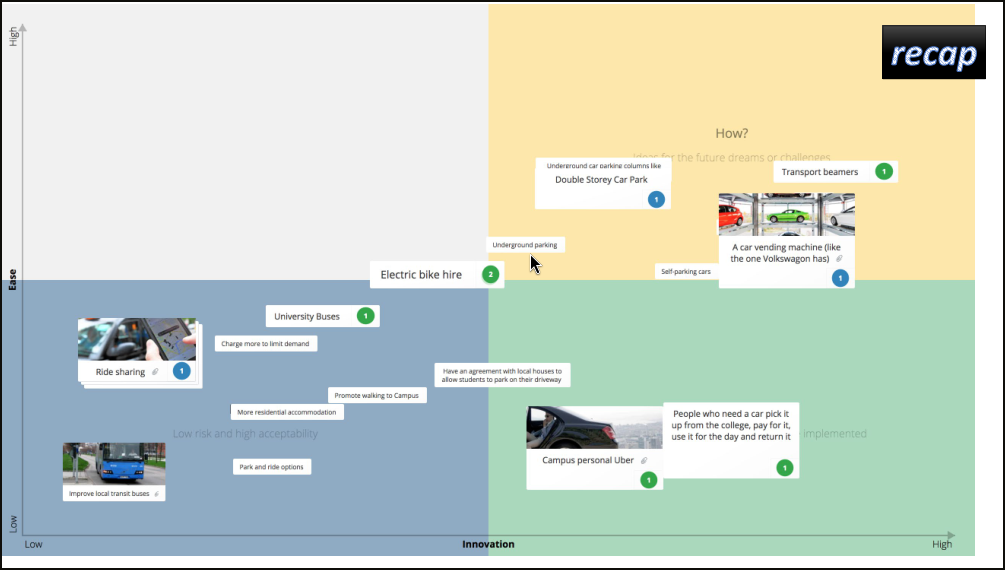
\includegraphics[width=\textwidth]{images/howwownowmatrix.png}
    \caption{Example ``How, Wow, Now'' Matrix}
\end{figure}

\subsection{The Process of IDEO}
$$
    \text{Understand} \rightarrow \text{Observe} \rightarrow \text{Visualise} \rightarrow \text{Evaluate} \rightarrow \text{Implement}
$$
\begin{enumerate}
    \item   \textbf{Understand} the market, the client, the technology.
    \item   \textbf{Observe} what confuses, what is hated, what is not satisfied.
    \item   \textbf{Visualise:} roleplay, storyboard, build an early stage prototype.
    \item   \textbf{Evaluate:} plan on several prototypes, concurrent engineering.
    \item   \textbf{Implement:} verify the final product works, commercialise, market.
\end{enumerate}

\subsection{The 5-Step Creative Process}
Creativity is a process that can be developed \& improved:
\begin{enumerate}
    \item   \textbf{Objective Finding:} stay focused on the ideal state you want to create, rather than just the
            solution to the problem.
            Identify what you want to happen when you solve the problem.
            \begin{itemize}
                \item   What are all of the problems that you would need to be solved for that ideal state to   
                        come true?
                \item   What solutions would you need to get for each of those problems?
                \item   Where can you find those solutions?
            \end{itemize}

            It is important \& useful to differentiate between the problem you are trying to solve and the 
            outcome that you are trying to achieve.

    \item   \textbf{Data Gathering:} the search for insight starts with the exercise of data collection and ends
            with the exercise of deciding which data is vital, interesting, \& insightful.
            \begin{itemize}
                \item   What is the recent history of this problem?
                \item   What has made it a problem?
                \item   Who are the people who will benefit from this solution?
                \item   What has been successful to this point and why?
                \item   What has failed to this point and why?
                \item   What hasn't been tried to this point and why?
                \item   What are the obstacles that stand in your way?
                \item   What obstacles might arise?
                \item   What are the restrictions inherent to this problem?
                \item   How do you want people to feel when they experience the solution?
            \end{itemize}

    \item   \textbf{Problem Design:} after identifying objectives \& gathering data, determine whether the 
            original problem is still the right problem to solve.
            Ask yourself ``will solving this problem lead to my objective?''; if so, move to the ideation stage,
            otherwise alter the problem or design a new one.

    \item   \textbf{Ideation:} don't solve the problem during ideation; generate as many possibilities as possible
            and leave the judgement of those possibilities for the next stage.

    \item   \textbf{Selection:} be very specific about what constitutes a solution to your problem and be 
            ruthless in determining which ideas meet those criteria.
            \begin{enumerate}[label=\roman*.]
                \item   Identify selection criteria, e.g. ``The solution will work if it...''.
                \item   Improve potential ideas. Every possible solution must be actionable.
                \item   Apply the selection criteria. Be merciless when choosing the solution.
            \end{enumerate}
\end{enumerate}

Each step is critical in developing innovative solutions.

\end{document}
